%% This is file `prletters-template.tex',
%%
%% Copyright 2013 Elsevier Ltd
%%
%% This file is part of the 'Elsarticle Bundle'.
%% ---------------------------------------------
%%
%% It maygupta2016synthetic be distributed under the conditions of the LaTeX Project Public
%% License, either version 1.2 of this license or (at your option) any
%% later version.  The latest version of this license is in
%%    http://www.latex-project.org/lppl.txt
%% and version 1.2 or later is part of all distributions of LaTeX
%% version 1999/12/01 or later.
%%
%% The list of all files belonging to the 'Elsarticle Bundle' is
%% given in the file `manifest.txt'.
%%
%% Template article for Elsevier's document class `elsarticle'
%% with harvard style bibliographic references
%%
%% $Id: prletters-template-with-authorship.tex 69 2013-07-15 10:15:25Z rishi $
%%
%% This template has no review option
%%
%% Use the options `twocolumn,final' to obtain the final layout
\documentclass[times,twocolumn,final,authoryear]{elsarticle}

%% Stylefile to load PR Letters template
\usepackage{prletters}
\usepackage{framed,multirow}

%% The amssymb package provides various useful mathematical symbols
\usepackage{amssymb}
\usepackage{latexsym}

%% �������ϵ�
%\usepackage{graphicx}
%\usepackage{booktabs}
%\usepackage{subfig}
\usepackage{amsmath,amssymb}
%\usepackage[lined,boxed,commentsnumbered]{algorithm2e}
\newcommand{\tabincell}[2]{\begin{tabular}{@{}#1@{}}#2\end{tabular}}
%% �������ϵ�
\usepackage{algorithm, algorithmic}
\usepackage{cite}

% Following three lines are needed for this document.
% If you are not loading colors or url, then these are
% not required.
\usepackage{url}
\usepackage{xcolor}
\definecolor{newcolor}{rgb}{.8,.349,.1}
\def\sep{,\space}

\journal{Pattern Recognition Letters}

\begin{document}

\ifpreprint
  \setcounter{page}{1}
\else
  \setcounter{page}{1}
\fi

\begin{frontmatter}

\title{A coarse-to-fine scene text detection method based on Skeleton-cut detector and Binary-Tree-Search based rectification}

\author[1]{Xiang \snm{He}}
\ead{hexiang@stu.xjtu.edu.cn}

\author[1]{Yonghong \snm{Song}\corref{cor1}}
\cortext[cor1]{Corresponding author:
  Tel.: +86-15029930633}
\ead{songyh@mail.xjtu.edu.cn}

\author[2]{Yuanlin \snm{Zhang}}
\ead{ylzhangxian@mail.xjtu.edu.cn}

\address[1]{School of Software Engineering, Xi'an Jiaotong University, Xi'an 710049, China}

\address[2]{Institute of Artificial Intelligence and Robotics, Xi'an Jiaotong University, Xi'an 710049, China}

\begin{abstract}


Scene text detection has been a long standing hot and challenging research topic in pattern recognition. In this paper a novel coarse-to-fine text detection method is proposed to solve edge-adhesion problem. In coarse detection stage, Skeleton-cut detector is proposed. At first,8-Neighborhoods-Search is applied on skeletons map to find the adhesion junctions between text and background skeletons. Then junctions in disordered skeletons are picked out by hysteresis selection and cut to separate text skeletons from background. And the text skeletons are verified through a two-stage classifier to obtain the coarse detection result. In fine detection stage, bounding boxes of all these filtered skeletons are weighted accumulated to obtain the Static Skeleton Response(SSR). Then many finer text lines candidates can be calculated through the gradient operation to the SSR's horizontal projection. And the text rectification based on Binary-Tree-Search is proposed to find a path from text lines' search space to the fine detection result. Experimental results on ICDAR dataset, SVT dataset and MSRA-TD500 dataset demonstrate that our algorithm achieves state of art performance in scene text detection.

\\[5pt]

{\it Keywords:}
  Scene text \sep Coarse-to-fine \sep  Skeleton-cut detector\sep SSR and BTS
\end{abstract}

\end{frontmatter}
\unhbox\keybox
%\linenumbers

%% main text
\section{Introduction}
\label{sec:intro}
Text could convey valuable informations in scene images. Scene text detection and recognition have become an active direction in community driven by the huge demand for a variety of practical computer vision techniques such as automotive assistance, multilingual translation and image retrieval. Though studied extensively in recent years \citep{chen2004detecting,neumann2011method,wang2011end,
yao2012detecting,bissacco2013photoocr,ye2015text}, text detection in natural scenes is still quite challenging due to complex backgrounds, various texts and interferential factors \citep{yao2013rotation}.

For detecting text in scene images, previous works have utilized the connected component analysis (CCA) \citep{epshtein2010detecting,chen2011robust,yi2012localizing,
yi2013text,huang2013text,shi2013scene,zamberletti2014text} and sliding window approach \citep{bissacco2013photoocr,kim2003texture,hanif2009text,lee2011adaboost,wang2012end} as two classes of mainstream methods. The latter category includes exhaustive search based methods which could achieve high recall rates by shifting a window through every locations of a given scene image in multiple scales to detect texts. However, a large number of candidates generated from the through scanning of windows would give rise to intolerably heavy computations, and may result in a great deal of false positives in addition.

\begin{figure*}[htbp]
\centering
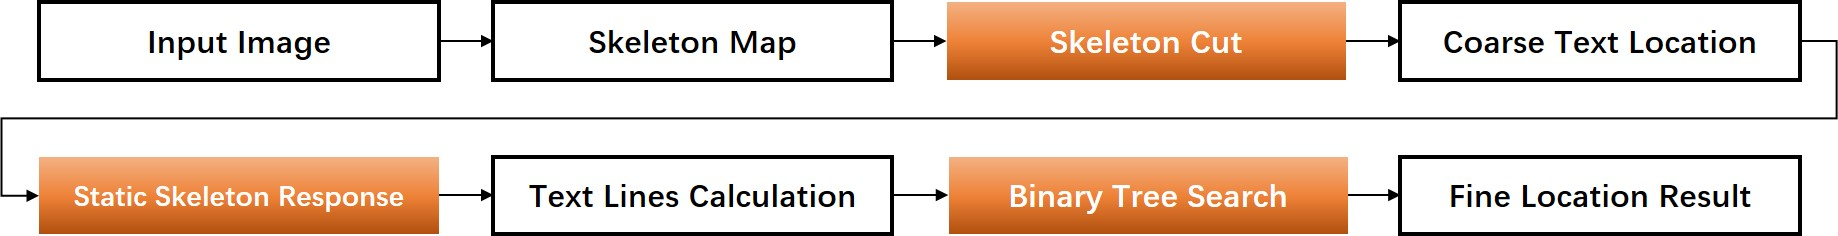
\includegraphics[width=0.95\linewidth]{./pic/flowchart3.jpg}
\label{fig.overview}
\caption{\footnotesize The flowchart of the proposed method: (top)Skeleton Cut Text Detector,(bottom)Text Recognition based on SSR and BTS.}
\end{figure*}

On the other hand, in those methods based on CCA, character candidates are extracted from the input scene image first. And majority of non-text in candidates are suppressed subsequently. In particular, Stroke Width Transform (SWT) or Maximally Stable Extremal Region (MSER) based methods have achieved outstanding performances on various test datasets due to their efficiency and stability. But even these representations might perform poorly under some severe conditions (e.g. low resolution, blur or non-uniform illumination), leading to low detection rate in practice.

Some recent text detector based on deep learning have achieved excellent results. \citet{Zhang2015Symmetry} exploits the symmetry property of character groups, and adopt CNN based classifiers to remove false positive. \citet{Zhang2016Multi} is the first method to train Fully Convolutional Network to predict the salient map of text regions. Inspired by SSD \citep{Liu2016SSD}, \citet{Liao2016TextBoxes} presents an end-to-end trainable fast scene text detector, named TextBoxes. And \citet{Shi2017Detecting} introduce a really fast oriented text detection method based on Segment Linking. Deep learning based methods obtained better detection performance, but are resource consuming.

In this paper we proposed an coarse-to-fine architecture including skeleton-cut detector and BTS based text rectification from top to bottom, as shown in Fig \ref{fig.overview}.

The main contributions of our method include: (1) In coarse detection stage, skeleton-cut detector is proposed to handle edge-adhesion problem via skeleton-junctions' detection and elimination; (2) In the stage of fine detection, SSR's projection and gradient is applied on coarse results to built the text lines' search space.(3)We proposed the BTS based text rectification, which aims to find a path from candidate text lines' search space to optimized detection results.

 The rest of the paper is organized as follows: Coarse text detection based on skeleton-cut is described in section \ref{sec:skel}. Details of fine text detection including SSR and BTS is  described in section \ref{sec:ser}. Evaluation on public benchmarks is shown in section \ref{sec:experiment}. Eventually, conclusions are stated in section \ref{sec:conclusion}.

\begin{figure}[htbp]
\centering

\includegraphics[width=7.5cm]{./pic/pipeline1.jpg}
\begin{minipage}[t]{0.3\linewidth}
\centerline{\footnotesize (a)Input image}
\end{minipage}
\begin{minipage}[t]{0.3\linewidth}
\centerline{\footnotesize (b)Edge response}
\end{minipage}
\begin{minipage}[t]{0.3\linewidth}
\centerline{\footnotesize (c)Text skeleton}
\end{minipage}

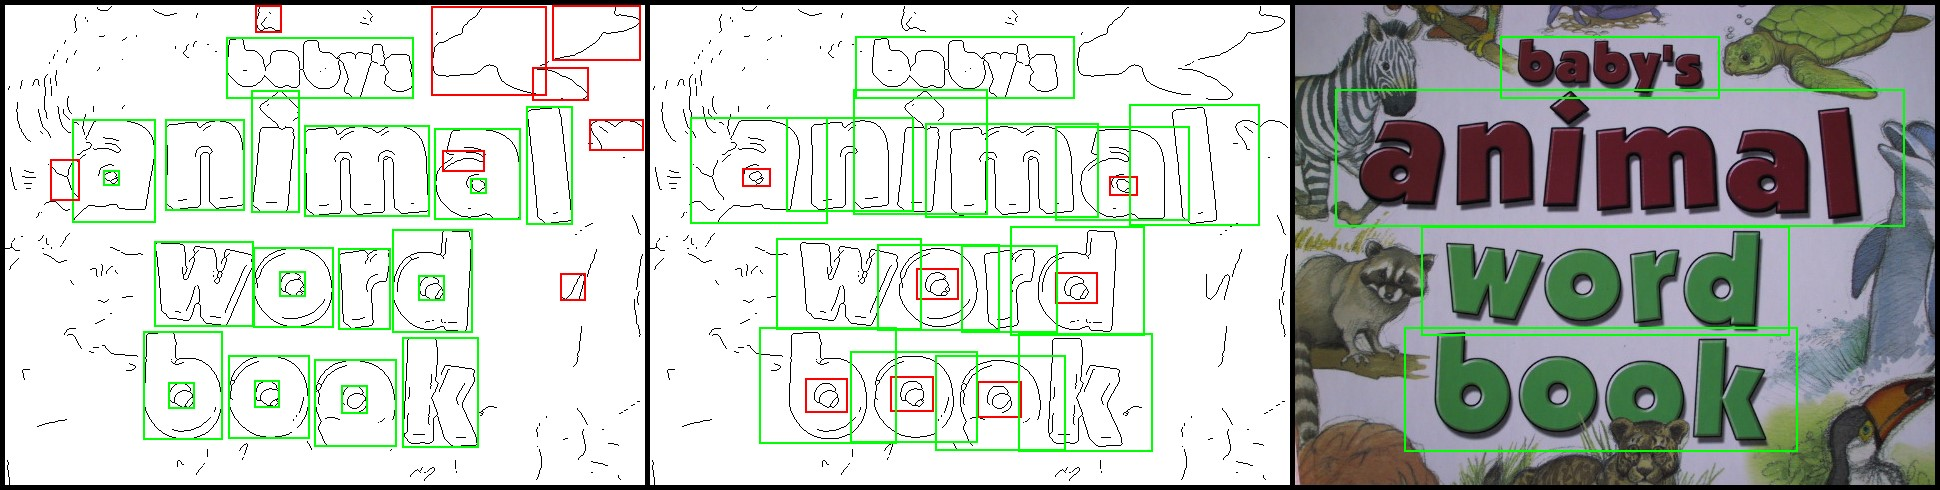
\includegraphics[width=7.5cm]{./pic/pipeline2.jpg}
\begin{minipage}[t]{0.3\linewidth}
\centerline{\footnotesize (d)Skeleton cutting}
\end{minipage}
\begin{minipage}[t]{0.3\linewidth}
\centerline{\footnotesize (e)Skeleton grouping}
\end{minipage}
\begin{minipage}[t]{0.3\linewidth}
\centerline{\footnotesize (f)Detection result}
\end{minipage}
\caption{The pipeline of Skeleton-cut text detector.}
\label{fig.pipeline2}
\end{figure}

\section{Coarse text detection based on Skeleton-cut}
\label{sec:skel}

Skeleton-cut detector's full process is illustrated as Fig \ref{fig.pipeline2}. In the first step of the proposed approach, we employ the Structured-forest edge detector described in \citep{dollar2015fast} on the input image $I$ (see Fig \ref{fig.Skel_Junc}(a)) to obtain the sparse edge response   (see Fig \ref{fig.Skel_Junc}(b)). Each pixel of the response   is labeled with a value indicating the probability of the pixel belonged to an edge. While the structural information of text could be well represented by edge response, it is difficult to extract text edges from response because of the edge-adhesion problem: In the response, some text edges which are connected to back-ground edges are hard to identify.

\begin{figure}[htbp]
\centering

\includegraphics[width=7.5cm]{./pic/Skel_Junc.jpg}

\begin{minipage}[t]{0.24\linewidth}
\centerline{\footnotesize (a)Image}
\end{minipage}
\begin{minipage}[t]{0.24\linewidth}
\centerline{\footnotesize (b)Response}
\end{minipage}
\begin{minipage}[t]{0.24\linewidth}
\centerline{\footnotesize(c)Map}
\end{minipage}
\begin{minipage}[t]{0.24\linewidth}
\centerline{\footnotesize (d)Skeleton}
\end{minipage}

\caption{The procedure of Skeleton-junctions detection.}
\label{fig.Skel_Junc}
\end{figure}

\subsection{Text Skeleton's Cutting}

To solve the edge-adhesion problem, we first segment the edge response through incremental thresholds to get a series of binary edge map $M$ (for instance, one of the maps is illustrated as Fig \ref{fig.Skel_Junc}(c)). And then skeleton-junction's detection and elimination are performed on these maps to cut text-edges out from background.

CNN based object skeleton detection methods \citep{Shen2016DeepSkeleton,Shen2016Object} can detect text skeletons. However, on the basis of edge map, a lightweight method is proposed in this paper to obtain candidate text skeletons: Given map $M$, we construct the presentation skeletons by thinning operation \citep{Lam2002Thinning}. The resulting skeletons $S$ are shown as the minimally connected 1-pixel-width strokes or rings in Fig \ref{fig.Skel_Junc}(d).

\begin{figure}[htbp]
\centering
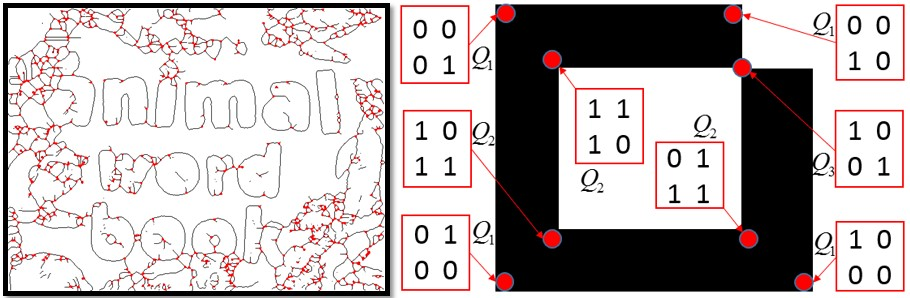
\includegraphics[width=7.5cm]{./pic/Euler_Num.jpg}
\begin{minipage}[t]{0.48\linewidth}
\centerline{\footnotesize (a)Disordered edge skeleton}
\end{minipage}
\begin{minipage}[t]{0.48\linewidth}
\centerline{\footnotesize (b)Quads detected on skeleton}
\end{minipage}
\caption{Select the most distinct skeleton based on Euler-number calculation.}
\label{fig.Euler_Num}
\end{figure}

After text skeletons construction, a number of skeleton-junctions $J$ could be obtained on skeletons $S$ by equation \ref{eq:SkelJunc}:

\begin{equation}
J=\left\{ p|n(p)=\sum_{k=1}^8x_k>t \right\},
\label{eq:SkelJunc}
\end{equation}

Where $n(p)$ is the sum values of the pixel $p$' neighbors, $t$ is a threshold value used for extracting skeleton-junctions and is experimentally set as $t=3$. The resulting skeleton-junctions $J$ are illustrated as red points in Fig \ref{fig.Skel_Junc}(d).

Notice that some skeletons are disordered and not suitable for skeleton-junction's detection and elimination. To avoid getting the disordered skeletons as shown in Fig \ref{fig.Euler_Num}(a), we employ Euler-number calculation to select the most distinct skeleton $skel$ from $S$.

Euler number, a scalar that specifies the number of objects in the region minus the number of holes in those objects, could indicate whether a skeleton is disordered or not. We first detect quads $Q_1,Q_2$ and $Q_3$ on $skel$ (see Fig \ref{fig.Euler_Num}(b)), and then calculate the Euler number of $skel$ using Equation \ref{eq:Euler_Num}.

\begin{equation}
\eta(skel)=\frac{n(Q_1)-n(Q_2)+2n(Q_3)}{4},
\label{eq:Euler_Num}
\end{equation}

Where quads $Q_1,Q_2$ and $Q_3$ are $2 \times 2$ pixel patterns, and $n(Q)$ is the number of $Q$. Next, in order to adaptively select the most suitable skeleton $skel$ in the skeletons set $S$, hysteresis selection is proposed: only $skel$ with moderate Euler number $\eta$ and skeleton junctions number $J$ could be preserved. By using hysteresis selection, more information(e.g. skeleton and junctions' constrains) gathered in later stages are taken into consideration to select best skeleton result. This selection not only reduce the computational cost introduced by handling the disordered skeleton, but also prevent $skel$ from being segmented into too-small fragments, which correct the cumulative error to an extent. Finally we eliminate the skeleton-junctions of selected $skel$ to cut text skeletons out from background and therefore address the edge-adhesion problem.

\begin{figure}[htbp]
\centering
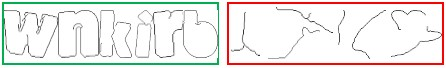
\includegraphics[width=7.5cm]{./pic/skel.jpg}
\begin{minipage}[t]{0.48\linewidth}
\centerline{\footnotesize (a)Text skeletons}
\end{minipage}
\begin{minipage}[t]{0.48\linewidth}
\centerline{\footnotesize (b)Background skeletons}
\end{minipage}
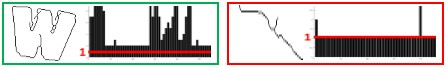
\includegraphics[width=7.5cm]{./pic/Concen_ratio.jpg}
\centerline{\footnotesize (c) Concentration ratio of text skeleton and background skeleton}
\caption{Text has higher cohesion degree than background.}
\label{fig.skel}
\end{figure}

\subsection{Text Skeleton's Filtering}
In the second step of Skeleton-cut detection, we filter out non-texts using two-stage classifier. Now let us consider the difference between text skeletons and other skeletons. As we can see in Fig \ref{fig.skel}(a-b), background skeletons are relatively straight and diffused, while text skeletons are rather curve and agglomerate. Based on this observation, most of non-texts could be eliminated by geometric constraints. Remaining text proposals are hard to distinguish, thus need to be classified by a CNN classifier inspired by \citep{wang2012end}.

Majority of non-text skeletons are removed in the first stage by geometric constraints such as aspect ratio, eccentricity, solidity and extent. In this paper we proposed a simple but effect constraint namely concentration ratio, which is the ratio of the $skel_{ol}$'$s$ length to the $skel$'$s$ length. We form this constraint mathematically as equation \ref{eq:ConRatio},

\begin{equation}
C(skel)=\frac{length(skel_{ol})}{length(skel)},
\label{eq:ConRatio}
\end{equation}

Where $skel_{ol}=skel(sum_{ver}(skel)>1)$is defined as the overlapped part of $skel$, and $Sum_{ver}(skel)$ is a vector obtained by adding up the values of $skel$ in the vertical direction (see Fig \ref{fig.skel}(c)). Text often has higher concentration ratio $C(skel)$. Thus we can coarsely filter the candidate text skeletons by concentration ratio.

For further precise classification, we train a convolutional neural network including two convolutional layers with $n_1=96$ and $n_2=256$ filters respectively, two pooling layers and one fully-connected layer as illustrated in Fig \ref{fig.cnn}. Finally the network is trained discriminatively by squared hinge loss.

\begin{figure}[htbp]
\centering
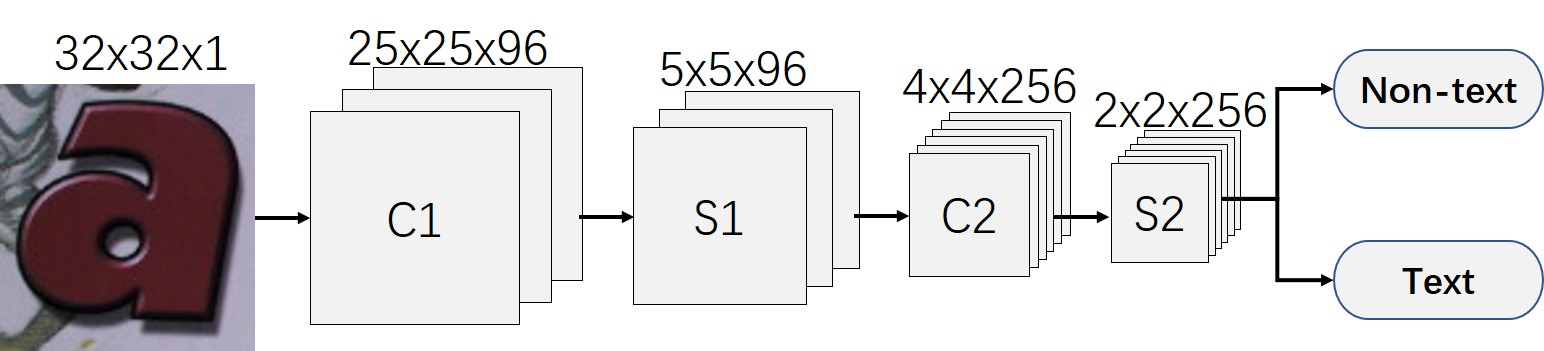
\includegraphics[width=7.5cm]{./pic/cnn.jpg}
\caption{The architecture of single-scale CNN classifier.}
\label{fig.cnn}
\end{figure}

In the testing stage, we first use Skeleton-cut detector to generate the text proposals $P$ and their bounding boxes. Instead of computing full-image-responses pyramid by multi-scale-sliding-window-based detection, in this paper we perform convolutional operation only on $P$ by single scale $s$, where $s=\left. height(B) \middle / 32 \right.$. Then the responses of the last layer are fed into the SVM classifier to score each proposal $p$ in $P$ . Finally false proposals with low confidence are rejected, giving the detection results including skeleton-boxes sets $B$ and their corresponding confidences $C$ .

\begin{figure}[htbp]

\begin{minipage}[t]{0.37\linewidth}
\centering
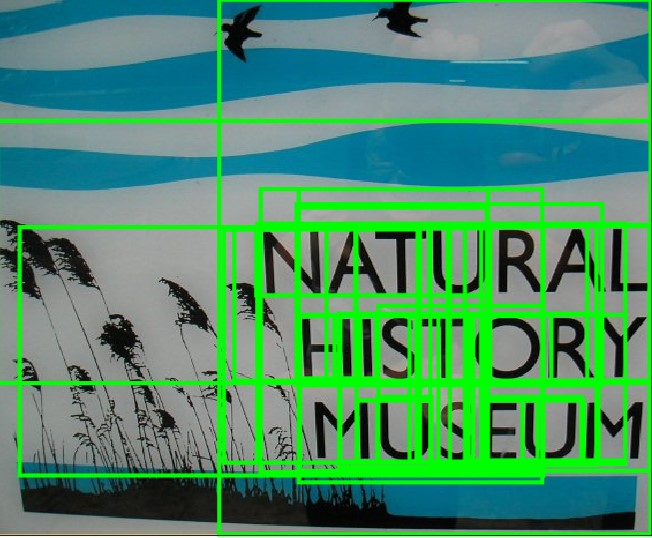
\includegraphics[width=\textwidth]{./pic/img_111-2.jpg}
\centerline{\footnotesize (a)Scene text image}
\end{minipage}
\begin{minipage}[t]{0.35\linewidth}
\centering
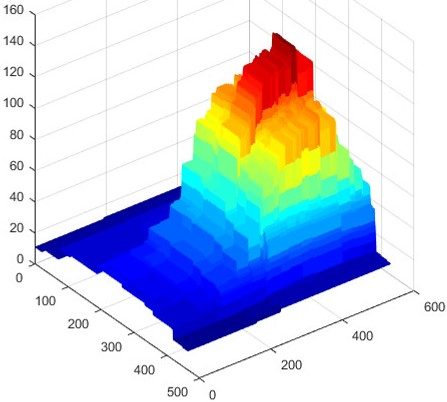
\includegraphics[width=\textwidth]{./pic/SSR1.jpg}
\centerline{\footnotesize (b)SSR}
\end{minipage}
\begin{minipage}[t]{0.25\linewidth}
\centering
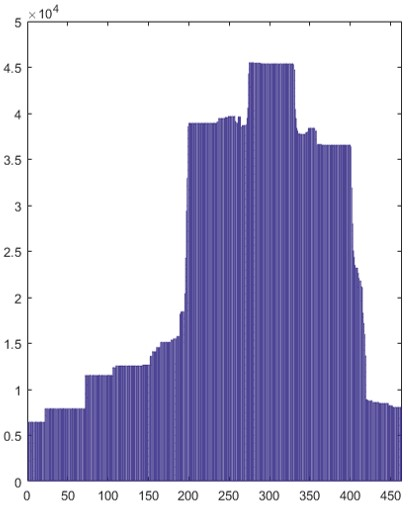
\includegraphics[width=\textwidth]{./pic/LTRSP2.jpg}
\centerline{\footnotesize (c)Horizontal Projection}
\end{minipage}
\caption{In SSR, text area is distinguished from background. And text lines could be separated from each other by horizontal projection.}
\label{fig.SSR}

\end{figure}

\section{Fine text detection based on SSR and BTS}
\label{sec:ser}

As shown in sec \ref{sec:skel}, coarse text detection result is obtained by skeleton-cut detector. But the result might not be very accurate due to the errors accumulated in the coarse detection process. To solve the error accumulation problem, text line rectification by binary binary tree search(BTS) is proposed.

\subsection{Search space's Construction by SSR}

First Static Skeleton Response(SSR) is proposed to enhance the difference of response intensity between text and background. Given a scene text image $g$ (see Fig \ref{fig.SSR}(a)), it's SSR $s$ is calculated based on Algorithm \ref{alg:SSR}.

\begin{algorithm}\small \renewcommand{\algorithmicrequire}{\textbf{Input:}}	\renewcommand{\algorithmicensure}{\textbf{Output:}}
	\caption{Statistic Skeleton Response(SSR)}
	\label{alg:SSR}
	\begin{algorithmic}[1]
		\REQUIRE scene text image $g$
		\ENSURE $g$'$s$ Statistic skeleton response $s$
        \STATE Skeleton-cut detector is applied on $g$ to get it's detection results: Skeleton-boxes set $B$ and Confidence set $C$.
		\REPEAT
        \STATE $rs:=\left\{ b \times c  |\,b \in B, c \in C\right\}$
        \STATE $s:=s\cup rs,B:=B / b,C:=C / c$
        \UNTIL{$B=\varnothing$}
	\end{algorithmic}
\end{algorithm}

where $rs$ is the response slice whose floor area is $b$ and height is $c$. $b$ is one of skeleton-boxes $B$, and $c$ is $b's$ corresponding confidence score. Finally all these response slices $rs$ stack up to build the SSR $s$ (see Fig \ref{fig.SSR}(b)).

\begin{figure}[htbp]
\begin{minipage}[t]{0.32\linewidth}
\centering
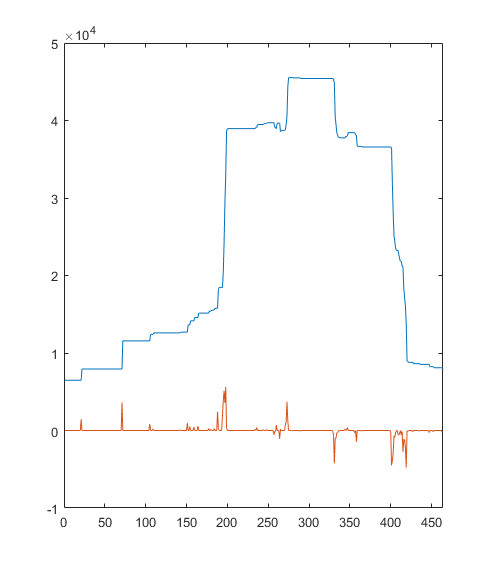
\includegraphics[width=\textwidth]{./pic/gradient.jpg}
\centerline{\footnotesize (a)Gradient on HP}
\end{minipage}
\begin{minipage}[t]{0.32\linewidth}
\centering
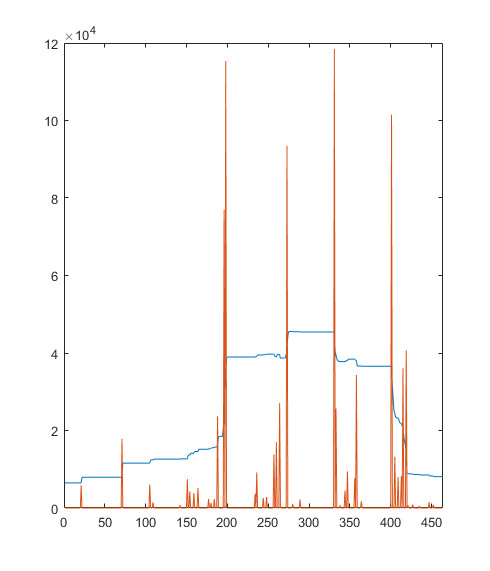
\includegraphics[width=\textwidth]{./pic/unified.jpg}
\centerline{\footnotesize (b)Absolute value of Gradient}
\end{minipage}
\begin{minipage}[t]{0.32\linewidth}
\centering
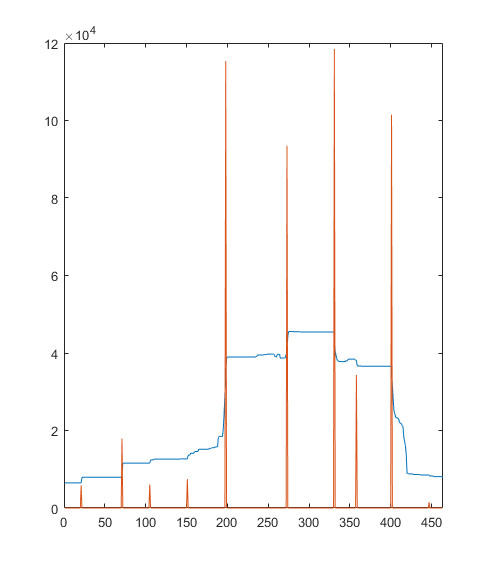
\includegraphics[width=\textwidth]{./pic/NMS.jpg}
\centerline{\footnotesize (c)NMS}
\end{minipage}
\caption{ Coarsely localizing text lines by gradient and nms operation.}
\label{fig.CLC}
\end{figure}

 Then SSR $s's$ horizontal projection $hp$ (Fig \ref{fig.SSR}(c))is calculated as equation \ref{eq:Cross-sec}, where $h,w$ are the height and width of $s$.

\begin{equation}
hp= \left\{ \sum_{j=1}^w s_{ij} \, | \, i=1,2,...,h;j=1,2,...,w \right\},
\label{eq:Cross-sec}
\end{equation}

And gradient $g$ is obtained on $hp$, which is illustrated as red pulse lines in Fig \ref{fig.CLC}(a). Gradient $g$ represents the variation degree of response, and the longer red pulse line $l$ in $g$ indicates that it's more likely to have a border between text and background near $l$. To facilitate the observation and analysis, the absolute value of $g$ is performed, and the coordinates of $g$ and $hp$ are unified (see Fig \ref{fig.CLC}(b)). Finally NMS operation is taken on $g$ to remove invalid red lines with low gradient magnitude, giving the candidate text lines set $L$(see Fig \ref{fig.CLC}(c)).

Given $L$ which has $m$ red lines $l_i,i=1,2,...,m$ in Fig \ref{fig.searchspace}(b), $m$-1 strips (the area between two neighbor red lines $l_i$ and $l_{i+1}$) can be found in scene text image. Now the task of this stage is that regarding all the combinations of strip zones as search space firstly, and then selecting the optimal strips set which precisely cover the text area from the space.

 \begin{algorithm}\small
	\renewcommand{\algorithmicrequire}{\textbf{Input:}}
	\renewcommand{\algorithmicensure}{\textbf{Output:}}
	\caption{Recursively build the Binary Tree}
	\label{alg:BBT}
	\begin{algorithmic}[1]
		\REQUIRE Lines $L's$ distances $LD=\left\{ld_1,ld_2,...,ld_m\right\}$ and confidences $LC=\left\{lc_1,lc_2,...,lc_m\right\}$
		\ENSURE Binary Tree $N's$ ranges $NR=\left\{nr_1,nr_2,...,nr_{2m-3}\right\}$, and values $NV=\left\{nv_1,nv_2,...,nv_{2m-3}\right\}$

      \STATE Initialization: \\
      \STATE \quad $i=0, \quad BuildBinaryTree(i,LD,LC)$

      \STATE function $BuildBinaryTree(i,LD,LC)$
        \\\STATE \quad $i=i+1$
        \\\STATE \quad $if \quad length(LD)==2 \quad then$
        \\\STATE \qquad $nr_{i}=[LD[1],LD[2]], nv_{i}=0$
        \\\STATE \qquad $return$
        \\\STATE \quad $end \ if$
        \\\STATE \quad $nr_{i}=[LD[1],LD[end]], nv_{i}=max(LC)$
        \\\STATE \quad $//$Suppose $lc_t$ is the max value in $LC$, and $t$ is $lc_t$'s index.
        \\\STATE \quad $//$We split $L$ into left set and right set at index $t$.
        \\\STATE \quad $LD_{l}=\left\{LD[1],...,LD[t]\right\}, LC_{l}=\left\{LC[1],...,LC[t]\right\}$
        \\\STATE \quad $BuildBinaryTree(i,LD_{l},LC_{l})$
        \\\STATE \quad $LD_{r}=\left\{LD[t],...,LD[end]\right\}, LC_{r}=\left\{LC[t],...,LC[end]\right\}$
        \\\STATE \quad $BuildBinaryTree(i,LD_{r},LC_{r})$
      \STATE end function

	\end{algorithmic}
\end{algorithm}

Suppose red line $l_i$ has two attributes: $ld_i$ and $lc_i$. $ld_i$ indicates the distance from the image's top to the $l_i$'s location(e.g. $ld_3$=$331_{px}$ in Fig \ref{fig.searchspace}(b). And $lc_i$ means the confidence of $l_i$, which is normalized from $l_i$'s gradient magnitude (e.g. $lc_3$=$0.987$ in Fig \ref{fig.searchspace}(b)). Then suppose $n$ is one of the nodes of the binary tree $N$. Node $n_i$ has two attributes: $nr_i$ and $nv_i$. $nr_i$ is the range of $n_i$, and $nv_i$ is the confidence value of $n_i$. For example, as we can see in Fig \ref{fig.searchspace}(a), $n_5$ is node rages from $l_3$ to $l_5$, whose value is assigned the confidence value of $l_4$.

\begin{figure}[htbp]
\centering
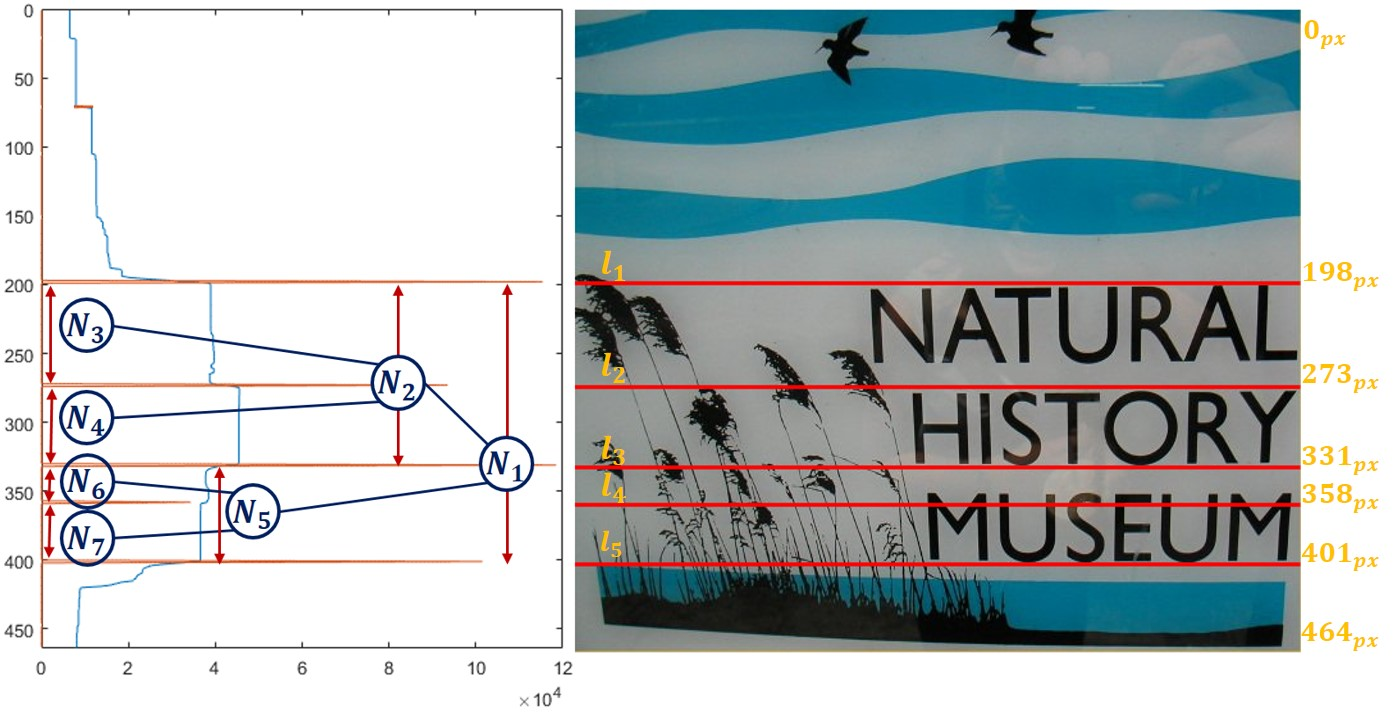
\includegraphics[width=0.48\textwidth]{./pic/BT6.jpg}
\begin{minipage}[t]{0.40\linewidth}
\centerline{\footnotesize (a)Binary tree search space.}
\end{minipage}
\begin{minipage}[t]{0.51\linewidth}
\centerline{\footnotesize(b)Candidate text lines on scene text image.}
\end{minipage}
\caption{  A binary tree which represents the search space is established from candidate text lines.}
\label{fig.searchspace}
\end{figure}

 Therefor a binary tree $N$ which represents the search space is established from lines $L$ by Algorithm \ref{alg:BBT}. Then space $N$ is stored in a table like Fig \ref{fig.searchtable}(a). In next section, the optimal path $P$ will be obtained from the space $N$ by the search strategy.

\subsection{Search strategy based on BTS}
\label{sec:bts}

Given search space $N$ which consist of $m$ nodes, paths set $P=\left\{ p_1,p_2,...,p_{(m-1)/2} \right\}$ is obtained by Algorithm \ref{alg:SBT}. Each path $p_i \in P$ is a nodes triple including parent node $np_i$, left node $nl_i$ and right node $nr_i$.

\begin{algorithm}\small
	\renewcommand{\algorithmicrequire}{\textbf{Input:}}	\renewcommand{\algorithmicensure}{\textbf{Output:}}
	\caption{Optimal paths searched on the Binary Tree}
	\label{alg:SBT}
	\begin{algorithmic}[1]
		\REQUIRE Nodes $N=\left\{n_1,n_2,...,n_m\right\}$, each node $n_x \in N$ has its corresponding attributes: range $nr_x$ and value $nv_x$.
		\ENSURE Paths  $P=\left\{p_1,p_2,...,p_{(m-1)/2}\right\}$, each path $p_{i} \in P$ is consist of  nodes triple $p_{i}=\left\{np_{i},nl_{i},nr_{i}\right\}$

      \STATE Initialization: $idx=0$
      \FOR{$i=1$ to $(m-1)/2$}

      \FOR{$j=1$ to $m$}
      \IF{$nv_j$ == $leastPositive(NV)$}
      \STATE $np_i = n_j, nv_j = 0, idx = j$
      \ENDIF

      \IF{$nr_j[1]$ == $nr_{idx}[1]$ and $nv_j$ == $0$}
      \STATE $nl_i = n_j, nv_j = -1$
      \ENDIF

      \IF{$nr_j[2]$ == $nr_{idx}[2]$ and $nv_j$ == $0$}
      \STATE $nr_i = n_j, nv_j = -1$
      \ENDIF

      \ENDFOR

      \STATE $p_{i}$ = $\left\{ np_{i},nl_{i},nr_{i} \right\}$

      \ENDFOR
	\end{algorithmic}
\end{algorithm}

 According to binary tree's property, $(m-1)/2$ iterations will be performed if there are $m$ nodes exists in $N$. In iteration $i$, $n_j \in N$ whose value $nv_j$ is the least positive number in $NV$ will be assigned to $np_i$. Then set $nv_j$ to 0 to convert $n_j$ into leaf node. And $n_x \in N$ whose range's beginning $nr_x[1]$ is equal to $n_j$'s range's beginning $nr_j[1]$ and value $nv_x$ is equal to 0 will be assigned to $nl_i$. Then set $nv_x$ to -1 to mark node $n_x$ as handled, which means $n_x$ wouldn't be considered in subsequent iterations. Similarly $n_t \in N$ is assigned to $nr_i$, and $nv_t$ is set as -1. After $(m-1)/2$ iterations, Paths set $P$ which consists of $(m-1)/2$ nodes triple $p$ is obtained.

\begin{figure}[htbp]
\centering
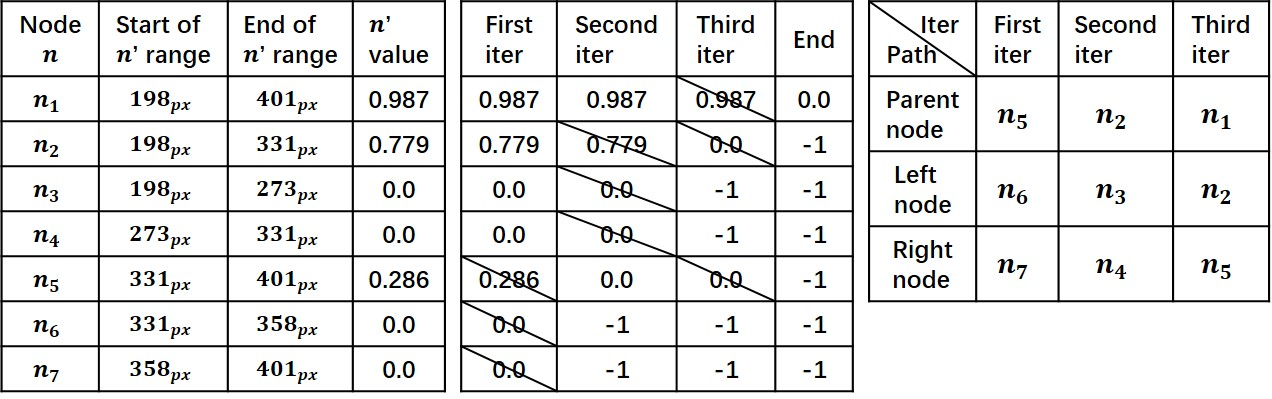
\includegraphics[width=0.48\textwidth]{./pic/search-table2.jpg}
\begin{minipage}[t]{0.33\linewidth}
\centerline{\footnotesize (a)BTS table.}
\end{minipage}
\begin{minipage}[t]{0.33\linewidth}
\centerline{\footnotesize(b)BTS iterations.}
\end{minipage}
\begin{minipage}[t]{0.26\linewidth}
\centerline{\footnotesize(C)BTS result.}
\end{minipage}
\caption{ A example of Binary Tree Search implement.}
\label{fig.searchtable}
\end{figure}

To comprehending the BTS algorithm mentioned above intuitively, an example is illustrated in Fig \ref{fig.searchtable}. First BTS table store the nodes of Binary Tree $N$ (as shown in \ref{fig.searchtable}(a)), $N$ has seven nodes). Then BTS algorithm is applied on search space $N$. After $(7-1)/2=3$ iterations (as shown in \ref{fig.searchtable}(b)), the paths result $P$ is obtained (as shown in \ref{fig.searchtable}(c)).

\begin{figure}[htbp]
\centering
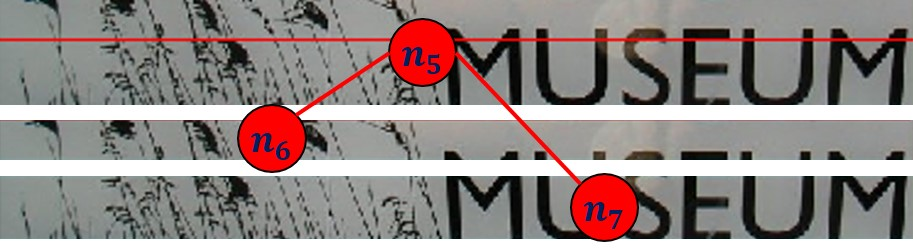
\includegraphics[width=7.5cm]{./pic/SEARCH-STRATEGY11.jpg}
\centerline{\footnotesize (a) A searched path. Each node represents a candidate text strip. }

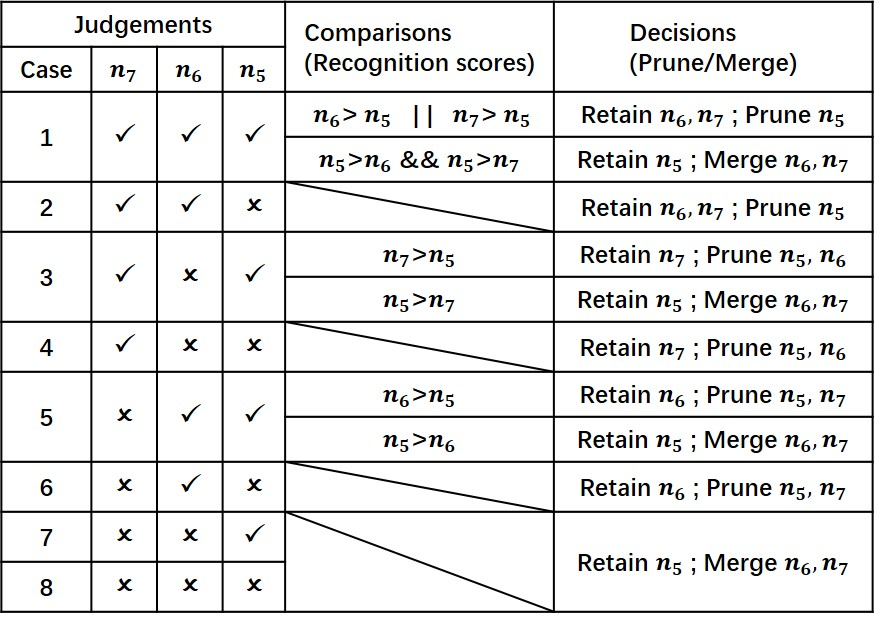
\includegraphics[width=7.5cm]{./pic/SEARCH-STRATEGY21.jpg}
\centerline{\footnotesize (b) Pruning and Merging strategy upon search path.}

\caption{ Strategy of obtaining the optimal text line by recognition result.}
\label{fig.searchstrategy}
\end{figure}

Finally search strategy will be performed on paths set $P$ to get optimal combination of text lines. Take $p_1=\left\{ np_1,nl_1,nr_1 \right\}=\left\{ n_6,n_7,n_5 \right\}$ as example(see Fig. \ref{fig.searchstrategy}(a)), there is only one decision in the following three strategies will be selected :(1)Retain $n_6$,then prune $n_7 $ and $n_5$; (2)Retain $n_7$,then prune $n_6 $ and $  n_5$; (3)Retain $n_5$ (which is same as merge $n_6$ and $n_7$),then prune $n_6$  and $n_5$. The selection procedure is based on nodes' recognition scores through a two-stage judgement which is illustrated in Fig. \ref{fig.searchstrategy}(b). We applied recognition model proposed in \citet{Jaderberg2016Reading} on node��s range $nr$ to obtain node's recognition score, then assign the score to node's value $nv$.

In the first state of judgement, the region of image that node $n_i$ represents is classified into text(marked as tick) or not (marked as cross) based on $n_i$'s recognition value $nv$: If $nv_i > 0$, then $n_i$ is judged as text region, else judged as non-text region. Thus one entry in $8=2^3$ cases is chosen. Then in the second stage, $nv$ of the entry mentioned above is comprised to get the final decision.

Next another path $p=\left\{ n_p,n_l,n_r \right\}$ is computed under the two-stage judgement to obtain it's corresponding decision. This procedure won't stop until all the paths in $P$ have been computed. Finally the optimal text detection result (that is the optimal path searched from the Binary Tree based Space) is obtained with the help of the text line's recognition score.

To verify the effect of BTS algorithm, our proposed method is compared with \citet{He2017Scene} on ICDAR and MSRA data sets. Skeleton cut detector and BTS based text line rectification are used in this proposed method, while only Skeleton cut detector is introduced in \citet{He2017Scene}. The experiment results in sec \ref{sec:experiment} show that the proposed method obtained better detection performance than \citet{He2017Scene}, which indicated that the BTS based text line rectification could correct the error accumulation problem to an extent.

\section{Experiment}
\label{sec:experiment}

\subsection{Datasets and Evaluation Protocol}

To evaluate our text detection method's performance, we run it on ICDAR 2003 (IC03), ICDAR 2011 (IC11), and ICDAR 2013(IC13) datasets, which respectively consist of 251, 255, and 233 fully annotated scene text images. These datasets are challenging for varieties of fonts, colors, scales and illuminations. Besides, MSRA-TD500 dataset is applied to validate the proposed method on multiple orientations and languages. And the Street View Text (SVT) dataset is consist of 249 road-side scenes with lots of noise and many unannotated words.

 Object count/area graphs \citep{wolf2006object} protocol is applied to measure recall, precision and f-measure as follows:

$recall = \frac {\sum_{i=1}^{|G|}Match_G(G_i,D,t_r,t_p)} {|G|}  ,   precision =\frac {\sum_{j=1}^{|D|}Match_G(D_j,G,t_r,t_p)} {|D|}$
And $f$ is the harmonic mean of precision and recall.

\subsection{Experimental Results}

\begin{table}[htbp]
\centering
\caption{Text Localization Performance on ICDAR 2013(\%).}
\begin{tabular}{l|l l l}
\hline
Method & Recall & Precision & F-score \\
\hline
\textbf{Proposed} & \textbf{89.2} & \textbf{76.5} & \textbf{82.3}\\
\citet{Cho2016Canny} & 78.4 & 86.2 & 82.1 \\
\citet{He2017Scene} & 76.2 & 86.7 & 81.1 \\
\citet{tian2015text} & 75.8 & 85.1 & 80.2 \\
\citet{zhu2016text} & 75 & 85 & 79 \\
\citet{Lu2015Scene} & 69.58 & 89.22 & 78.19 \\
\citet{gupta2016synthetic} & 66.30 & 94.80 & 78.00 \\
\citet{yin2014robust} & 65.11 & 83.98 & 75.89 \\
\citet{neumann2012real} & 64.84 & 87.51 & 74.49 \\
\hline
\end{tabular}
\label{tab.icdar13}
\end{table}

As seen in table \ref{tab.icdar13}, our proposed method achieves 89.2\% in recall, and 75.5\% in precision under the scheme of ICDAR 13. The state-of-art algorithm proposed by \citet{Cho2016Canny} obtained a harmonic mean of 81.1\% while our method achieves 82.32\%. The recall result of the proposed method is 89.2\%, which outperforms all outcomes of other text detection methods. The increased recall of ours is mainly due to the well designed skeleton proposal strategy and the establishment of candidate text lines�� search space. It is worth mentioning that the proposed detector delivers a fast algorithm for scene text detection which would bear much lower computational cost than CNN-based detector like \citet{tian2015text}. The dataset's average size is around 1,200 by 900 pixels. Our proposed algorithm cost 0.76 seconds to process an image(i.e. skeleton-cut detector, static skeleton response and binary-tree-based rectification). In addition, f-score would drop 2\% when the BTS based text rectification is removed (compare our previous method \citet{He2017Scene} to this proposed method ), which indicates that BTS rectification dose enhance the detection performance both on recall and precision rate.

\begin{table}[htbp]
\centering
\caption{Evaluation of character detection rate on ICDAR 2011.}
\begin{tabular}{l|l l }
\hline
Method & Num of candidates & Detection Rate \\
\hline
All ERs & 6,051,331 & 0.966 \\
\citet{matas2004robust} & 39,762 & 0.539 \\
\citet{sung2015scene} & 93,357 & 0.877  \\
\citet{Cho2016Canny} & 8,121 & 0.874 \\
\citet{He2017Scene} & 8,231 & 0.879 \\
\hline
\textbf{Proposed} & \textbf{7,137} & \textbf{0.892} \\
\hline
\end{tabular}
\label{tab.icdar11}
\end{table}

Table \ref{tab.icdar11} shows the quantitative comparison of character detection rate on ICDAR 2011 benchmark with \citet{sung2015scene} which propose the state-of-the-art ERs extraction method. The test set of ICDAR2011 includes 255 scene images and 6309 characters. Unlike the refined ERs of \citet{sung2015scene} that need further classification, our skeleton-cut detector proposed in \citet{He2017Scene} have eliminated more than 90\% of false candidates while preserving comparably high recall rate. And the skeleton-cut detector's detection rate is also superior than another state-of-art method proposed by \citet{Cho2016Canny} while detecting less false characters. This demonstrates that the representation skeleton's adaptability is stronger than that of ERs-based representations.

\begin{figure}[htbp]
\centering
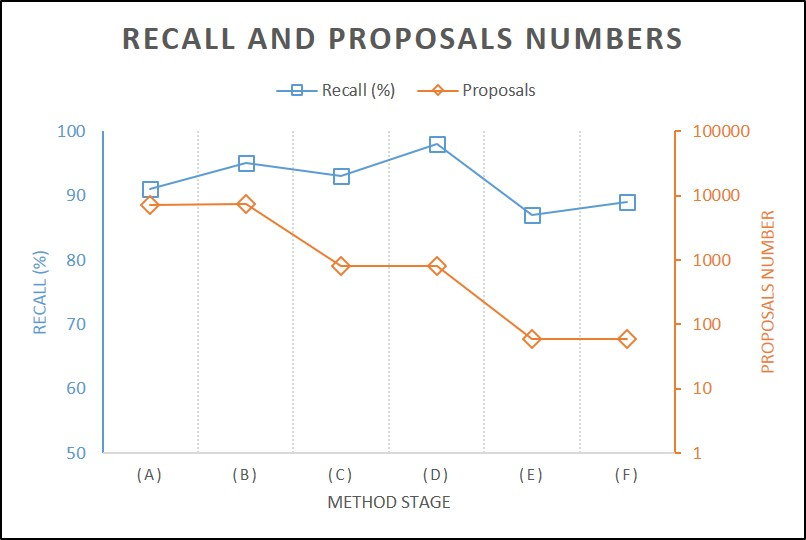
\includegraphics[width=7cm]{./pic/recall_proposals.jpg}
\caption{The recall and the average number of proposals per image on ICDAR2011 after each stage of the pipeline: (a)skeleton proposals, (b)skeleton cutting, (c)skeleton fitering, (d)candidate localization, (e)NMS, (f)BTS rectification. The recall computed is detection recall across the dataset at 0.5 overlap. }
\label{fig.rec_prop}
\end{figure}

In addition to skeleton-cut detector, text rectification based on BTS (binary tree search) is proposed in this paper to further reduce the amount of candidate characters. The
progression of detection recall and the number of proposals as the pipeline progresses can be seen in Fig \ref{fig.rec_prop}, which proved that combining BTS text rectification with skeleton-cut detector will improve precision of detection while obtaining a good recall result.

\begin{table}[htbp]
\centering
\caption{ Performance comparisons on MSRA-TD500 2011.}
\begin{tabular}{l|l l l}
\hline
Method & Recall & Precision & F-score \\
\hline
\textbf{Proposed} & \textbf{0.70} & \textbf{0.79} & \textbf{0.75} \\
\citet{He2017Scene} & 0.64 & 0.82 & 0.72 \\
\citet{yin2015multi} & 0.63 & 0.81 & 0.71 \\
\citet{kang2014orientation} & 0.62 & 0.71 & 0.66 \\
\citet{yin2014robust} & 0.61 & 0.71 & 0.65 \\
\citet{yao2012detecting} & 0.63 & 0.63 & 0.60\\
\hline
\end{tabular}
\label{tab.msra}
\end{table}

As shown in table \ref{tab.msra}, our proposed approach achieves recall 0.70, precision 0.79 and f-score 0.75 on MSRA-TD dataset, which outperform other methods significantly. In summary, our method could successfully detect text in natural images with multiple orientations and mixture of multi-language.

In table \ref{tab.deep}, deep learning based methods like TextBoxes \citep{Liao2016TextBoxes} have achieved excellent results. However, only high performance workstation and massive samples could effectively train the deep CNN proposed in above methods, which means the actual application scenario may be limited. Instead, skeleton-cut detector is a lightweight conventional text detector, which is designed to solve edge-adhesion problem, and could be run on ordinary machine (without a GPU) effectively.

%Inspired by SSD \citep{Liu2016SSD}, \citet{Liao2016TextBoxes} proposes an end-to-end trainable fast scene text detector, named TextBoxes

%However, they need a lot of training samples to fine-tune a good network. And Some samples should be customized to meet the training requirements, like \citet{Shi2017Detecting}

%These advanced deep learning based methods in Table \ref{tab.deep} obtain better detection scores than ours.

%Instead, a lightweight text detector named skeleton-cut is proposed in this paper

%Further, \citet{Shi2017Detecting} introduced Segments(oriented text boxes) and linking(relationship between adjacent segments) to train SSD-based network to detect multi-orientation text. %

%Instead, a lightweight text detector named skeleton-cut is proposed in this paper to solve edge-adhesion problem, which is easy to run on ordinary machine without GPU

\begin{table}[htbp]
\centering
\caption{ Performance comparisons with deep learning based methods on ICDAR 2013(\%).}
\begin{tabular}{l|l l l}
\hline
Method & Recall & Precision & F-score \\
\hline
\citet{Shi2017Detecting} & 83.0 & 87.7 & 85.3 \\
\citet{Liao2016TextBoxes} & 83.0 & 88.0 & 85.0 \\
\citet{Zhang2016Multi} & 78.0 & 88.0 & 83.0 \\
\textbf{Proposed} & 89.2 & 75.5 & 82.3\\
\citet{Liao2016TextBoxes}* & 74.0 & 86.0 & 80.0 \\
\citet{Zhang2015Symmetry} & 76.0 & 84.0 & 80.0\\
\hline
\end{tabular}
\label{tab.deep}
\end{table}

Some detection and skeleton results obtained from ICDAR and MSRA-TD500 datasets are showed in Fig \ref{fig.ruslts}. In the skeleton map results, we can see that most of the background skeletons adjoined to text via adjoin-junctions are eliminated. So that the text candidates could be separated from background to solve the edge-adhesion problem. In the detection results, our proposed detection method could robustly localise a range of texts, even there exists illumination, noise and Indistinguishable textures such as tree leaves, windows, and so on.

\begin{figure}[htbp]
\centering
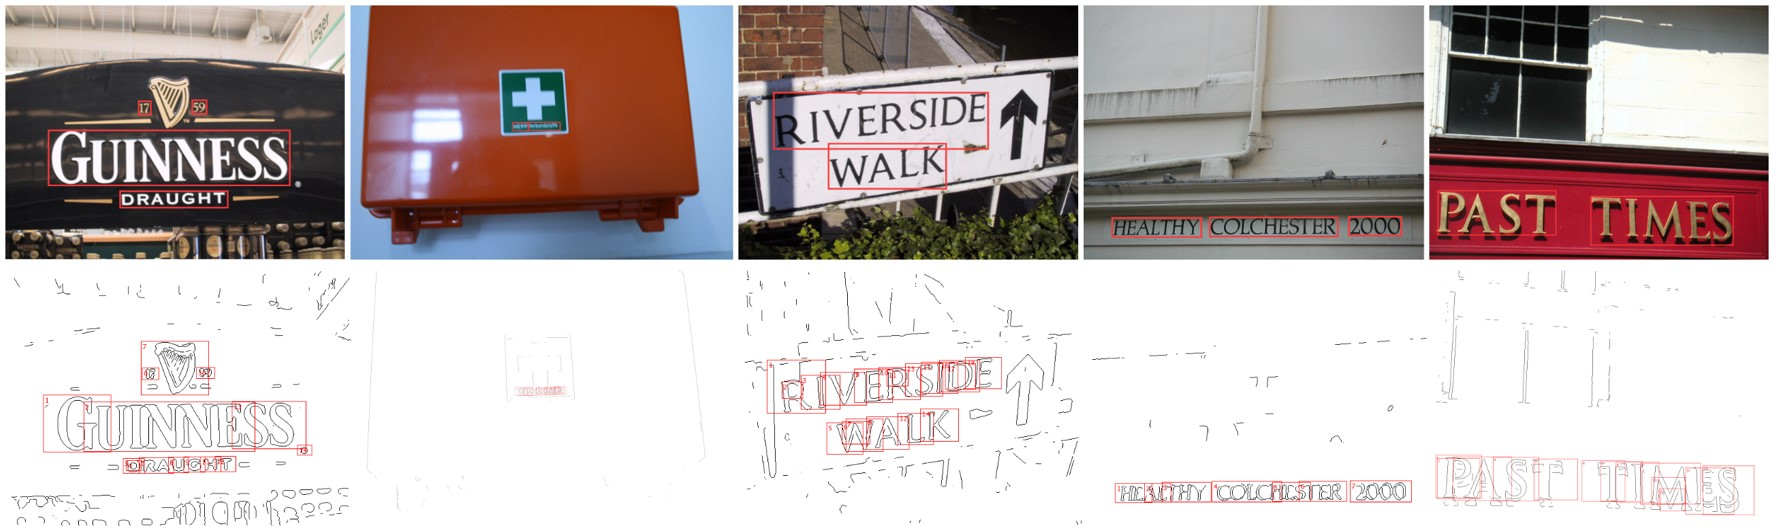
\includegraphics[width=8cm]{./pic/result4.jpg}
\centerline{\footnotesize (a)Detection results (top) and skeleton results (bottom) of ICDAR2013.}

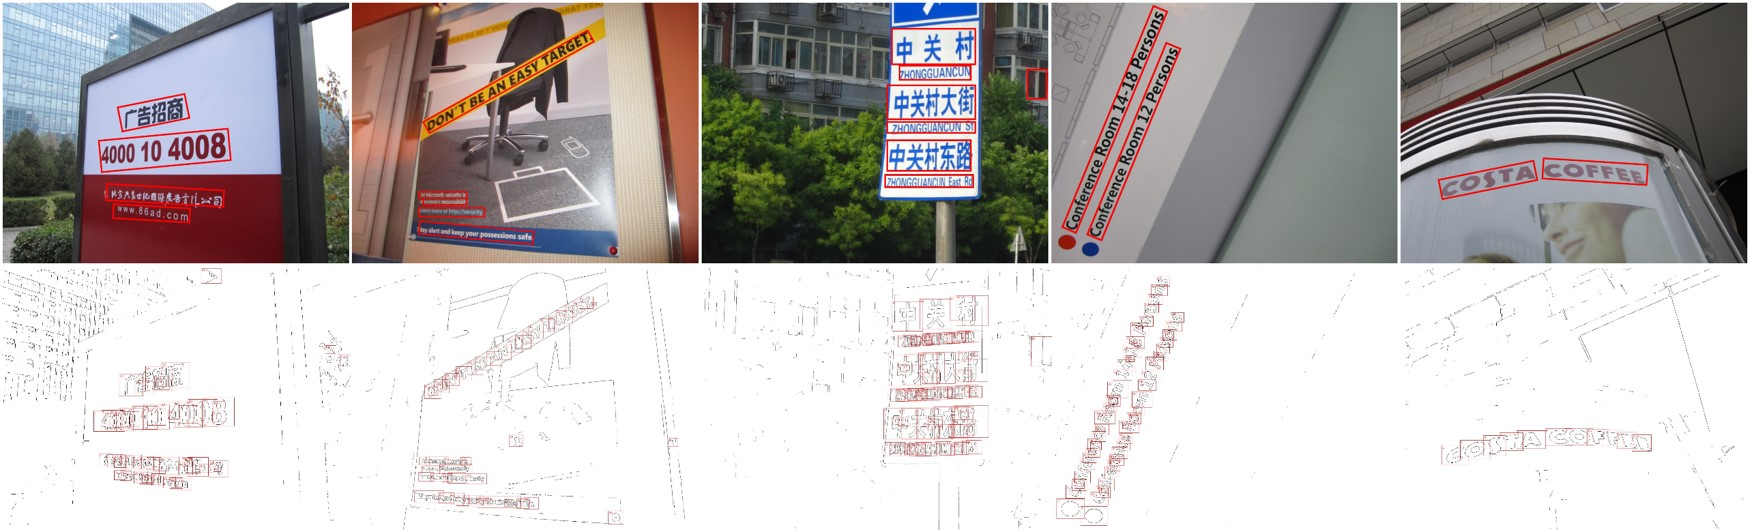
\includegraphics[width=8cm]{./pic/result4-2.jpg}
\centerline{\footnotesize (b)Detection results (top) and skeleton results (bottom) of MSRA-TD500.}

\caption{Sample results (detection and skeleton) on scene text detection datasets:  ICDAR 2013 and MSRA-TD500. Results are marked as red bounding boxes.}

\label{fig.ruslts}
\end{figure}

In the pipeline of BTS-based text rectification, a closer interaction of detection and recognition has be illustrated in section \ref{sec:bts}. These detection results could tightly surround the true text lines based on recognition scores. And the improved detection result could further enhance the accuracy of recognition in turn.

\begin{table}[htbp]\small
\centering
\caption{Comparison to previous methods for end-to-end text spotting.}
\begin{tabular}{l|l l l l l l l}
\hline
Model   & IC03 & SVT & IC11 & IC13  \\
\hline
\citet{neumann2011method}  & 41 & -- & -- & -- \\
\citet{neumann2013scene} & -- & -- & -- & 45 \\
\citet{Alsharif2013End} & 48 & -- & -- \\
\citet{Jaderberg2014Deep} & -- & 56 & -- & -- \\
\citet{Jaderberg2016Reading} & 78 & 53 & 76 & 76 \\
\citet{He2017Scene} & 78 & 53 & 75 & 77 \\
\textbf{Proposed} & 79 & 56 & 78 & 79 \\
\hline
\end{tabular}
\label{tab.recog}
\end{table}

Table \ref{tab.recog} shows our recognition��s results compared to other methods. Global F-score over images of the dataset has been reported in this table. Our recognition algorithm outperforms all these previous methods across all datasets. On IC03, IC11 and IC13, we improve the state-of-the-art by at least +2\%, achieving P/R/F of 0.85/0.72/0.79 respectively. Similarly improvement can been seen on SVT, where the result has been increased by +3\% to \citet{Jaderberg2016Reading}. Moreover, Fig \ref{fig.rec_prop} shows the proposals number/recall curves, in which we can see that our detection and recognition pipeline is able to maintain high recall, and the recognition��s score is a strong cue to the robustness of a detection.

\section{Conclusions}
\label{sec:conclusion}

In this paper, we have presented a novel coarse-to-fine framework for scene text detection. Skeleton-cut detector is proposed in coarse detection stage: First the adhesion-junctions between text and non-text skeletons are cut to separate text candidates from background. Then these candidates are filtered to obtain the coarse detection result. Subsequently in fine detection stage, filtered candidates' SSR is proposed to enhance the difference between text area and background. Then text lines' search space is built based on SSR's horizontal projection and gradient. And we propose BTS-based text rectification method to search a path from search space to the optimal detection result. Finally we evaluate the proposed method on public datasets and compared it with existing methods. Evaluation result shows that our method is comparable with state-of-art methods.

\bibliographystyle{model2-names}
\bibliography{refs}

\end{document}

%%
